\begin{icpcproblem}{D}{Diagrams \& Tableaux}{Arne Alex}{10}

A \emph{Young diagram} is an arrangement of boxes in rows and columns
conforming to the following rules:
\begin{itemize}
\item the boxes in each row and each column are
contiguous,
\item the left borders of all rows are aligned, and
\item each row is not longer than the one above.
\end{itemize}

Here are some examples of Young diagrams:

\begin{figure}[h]
\centering
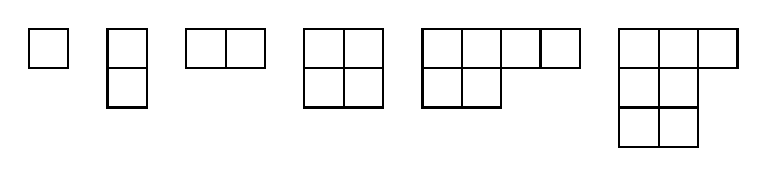
\begin{tikzpicture}
  \begin{scope}[scale=0.5,thick,minimum width=0.5cm,minimum height=0.5cm]
    \node[draw] at (0,0) {} ;

    \node[draw] at (2,0) {} ;
    \node[draw] at (2,-1) {} ;

    \node[draw] at (4,0) {} ;
    \node[draw] at (5,0) {} ;

    \node[draw] at (7,0) {} ;
    \node[draw] at (8,0) {} ;
    \node[draw] at (7,-1) {} ;
    \node[draw] at (8,-1) {} ;

    \node[draw] at (10,0) {} ;
    \node[draw] at (11,0) {} ;
    \node[draw] at (10,-1) {} ;
    \node[draw] at (11,-1) {} ;
    \node[draw] at (12,0) {} ;
    \node[draw] at (13,0) {} ;

    \node[draw] at (15,0) {} ;
    \node[draw] at (16,0) {} ;
    \node[draw] at (15,-1) {} ;
    \node[draw] at (16,-1) {} ;
    \node[draw] at (15,-2) {} ;
    \node[draw] at (16,-2) {} ;
    \node[draw] at (17,0) {} ;
  \end{scope}
\end{tikzpicture}
\end{figure}

A \emph{semi-standard Young tableau} for a given number $N$ is a Young diagram that has its boxes
filled according to the following rules:
\begin{itemize}
\item Each box contains a single integer
between $1$ and $N$, inclusive,
\item each integer is greater than or equal to the integer in the box to its left, and
\item each integer is strictly greater than the integer in the box above.
\end{itemize}

{\raggedright
Here is a list of all semi-standard Young
tableaux for $N=3$, based on a particular Young diagram:
\par}

\begin{figure}[h]
\centering
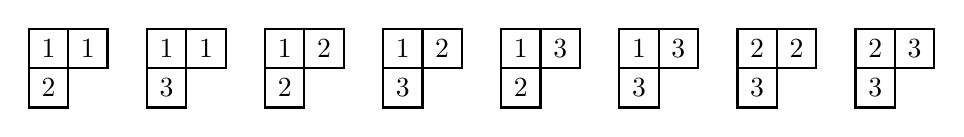
\begin{tikzpicture}
  \begin{scope}[scale=0.5,thick,minimum width=0.5cm,minimum height=0.5cm,inner sep=0cm]
    \node[draw] at (0,2) {1} ;
    \node[draw] at (0,1) {2} ;
    \node[draw] at (1,2) {1} ;

    \node[draw] at (3,2) {1} ;
    \node[draw] at (3,1) {3} ;
    \node[draw] at (4,2) {1} ;

    \node[draw] at (6,2) {1} ;
    \node[draw] at (6,1) {2} ;
    \node[draw] at (7,2) {2} ;

    \node[draw] at (9,2) {1} ;
    \node[draw] at (9,1) {3} ;
    \node[draw] at (10,2) {2} ;

    \node[draw] at (12,2) {1} ;
    \node[draw] at (12,1) {2} ;
    \node[draw] at (13,2) {3} ;

    \node[draw] at (15,2) {1} ;
    \node[draw] at (15,1) {3} ;
    \node[draw] at (16,2) {3} ;

    \node[draw] at (18,2) {2} ;
    \node[draw] at (18,1) {3} ;
    \node[draw] at (19,2) {2} ;

    \node[draw] at (21,2) {2} ;
    \node[draw] at (21,1) {3} ;
    \node[draw] at (22,2) {3} ;
  \end{scope}
\end{tikzpicture}
\end{figure}

Your task is to count how many semi-standard Young tableaux are possible, based on
a given Young diagram, with a given $N$.

\sectiontitle{Input}

Each test case consists of two lines. The first line of each test case specifies the Young diagram. This line starts with the number $k$ satisfying $1\le{}k \le{}7$, the number of rows, followed by $k$ positive integers $l_1,l_2,\ldots,l_k$. These integers specify the number of
boxes on each row of the Young diagram, and they satisfy $7\ge{}l_1\ge{}l_2\ge\cdots\ge{}l_k\ge{}1$.
The second line contains the integer $N$,
satisfying $k\le{}N\le{}7$.

\sectiontitle{Output}

For each test case, print one line containing the number of
semi-standard Young tableaux based on the given Young diagram, with the
given $N$.

\clearpage
\sampleio{sample}

\end{icpcproblem}
